\chapter{面向低动态水下场景的 ACO-AFDM 传输方案}
\label{chap:aco_afdm}

在低动态水下环境中，收发节点间相对运动通常较弱，因此由平台运动引起的多普勒扩展往往不是限制系统性能的主要因素。然而，悬浮颗粒引起的多重散射、有限空间中的反射以及非视距传播分量仍会造成明显的多径扩展，并进一步导致频率选择性衰落与符号间干扰。针对该类场景，本文提出一种面向强度调制/直接检测（Intensity Modulation/Direct Detection，IM/DD）架构的 ACO-AFDM 传输方案，旨在在满足光学发射物理约束的基础上，提高系统对低动态多径信道的适应能力。

与高动态场景相比，低动态 UWOC 的设计重点并不在于处理快速时变引起的严重多普勒耦合，而在于如何在有限发射功率和非负实信号约束下，提升系统对散射主导多径传播的鲁棒性。传统光 OFDM 体制虽然具有实现简单、工程基础较成熟等优势，但其仍建立在频域正交结构之上，当信道存在较明显时延扩展时，部分子载波容易受到深衰落和残余干扰影响，系统误码率性能会明显下降。AFDM 作为一种基于离散仿射傅里叶变换（Discrete Affine Fourier Transform，DAFT）的新型多载波体制，能够在变换域中获得更适合描述多径结构的信号表示，因此为低动态多径 UWOC 设计提供了新的思路。

需要指出的是，AFDM 原始形式面向复数基带系统，而 IM/DD 架构要求发射信号满足实值且非负约束，无法直接沿用传统复数域 AFDM 结构。基于此，本文将 ACO-OFDM 的奇数子载波映射与非对称限幅思想引入 AFDM 体制，在保持光学可实现性的同时，保留 AFDM 对多径传播更具适应性的结构优势，从而形成 ACO-AFDM 方案。

 

在传统 IM/DD 水下无线光通信系统中，发射端驱动光源的信号必须满足实数且非负的物理约束\cite{armstrongPowerEfficientOptical2006}。这意味着许多原本面向复数基带设计的高频谱效率调制方式，不能直接用于实际光学发射链路，而需要通过厄米特对称、直流偏置或限幅等方式完成适配。ACO-OFDM 正是在这一背景下发展起来的典型方案，其通过仅在奇数子载波上加载有效数据，并对时域双极性信号进行非对称限幅，实现了对非负约束的满足，同时具备较好的光功率效率\cite{dissanayakeComparisonACOOFDMDCOOFDM2013}。

然而，低动态 UWOC 的困难并不只来自信号的非负约束。在浑浊水体、近岸环境或受限空间条件下，光子在传播过程中会经历显著的吸收与散射，非视距分量和多重散射分量会形成具有不同传播时延的到达路径。这种传播特性虽然未必伴随很强的多普勒扩展，却会带来明显的时延扩展和频率选择性衰落。当系统带宽较大、符号周期较短时，这些失真将直接削弱传统光 OFDM 体制的正交解调优势，并增加接收端检测难度\cite{jaruwatanadilokUnderwaterWirelessOptical2008, yangAdvancementsUnderwaterOptical2024}。

从波形设计角度看，若仍完全沿用传统 OFDM 框架，则系统性能在较强多径条件下会受到明显限制。特别是在 ACO-OFDM 中，虽然奇数子载波映射与限幅结构能够较好满足 IM/DD 的发射要求，但其本质仍是基于傅里叶正交基进行信号展开。当频率选择性衰落增强时，各子载波上的信道响应不再均衡，部分频率位置会更易受到深衰落影响，从而使误码率性能下降。因此，针对低动态浑浊多径场景，仅依靠传统光 OFDM 结构很难同时兼顾非负实信号约束与多径鲁棒性。

AFDM 基于 DAFT 构造信号，可在等效变换域中获得更适合描述多径结构的表示形式，从而提高系统对频率选择性信道的适应能力\cite{bemaniAFDMFullDiversity2021}。其核心优势在于，通过引入啁啾相位结构，信号在经历路径时延后可在 DAFT 域中呈现更具规律性的分布特征，为后续信道分离与检测创造条件。基于此，本文将 AFDM 引入光学 IM/DD 系统，结合 ACO 机制设计 ACO-AFDM 传输方案，以兼顾非负实信号约束与多径鲁棒性。

需要强调的是，本文研究的低动态场景并非完全静态环境，而是以“多径主导、时变较弱”为主要特征的代表性 UWOC 传播条件。在此场景下，系统设计应优先关注多径扩展、频率选择性衰落及其对光学非负多载波体制的影响。因此，本章的核心目标是：在 IM/DD 架构下构建可实现的 ACO-AFDM 系统模型，分析其参数设计约束，并通过仿真验证其在低动态多径水下信道中的性能优势。

\section{ACO-AFDM 系统模型构建} 
\label{sec:aco_afdm_model}

本节建立所提 ACO-AFDM 系统的发射端、信道与接收端模型。系统完整框图如图~\ref{fig:aco_afdm_flow} 所示。与传统 ACO-OFDM 相比，所提方案的关键区别在于将傅里叶基替换为适配低动态多径场景的 AFDM 结构，并通过相应的实值化与限幅设计使其能够应用于 IM/DD 水下光链路。

\begin{figure}[htbp]
    \centering
    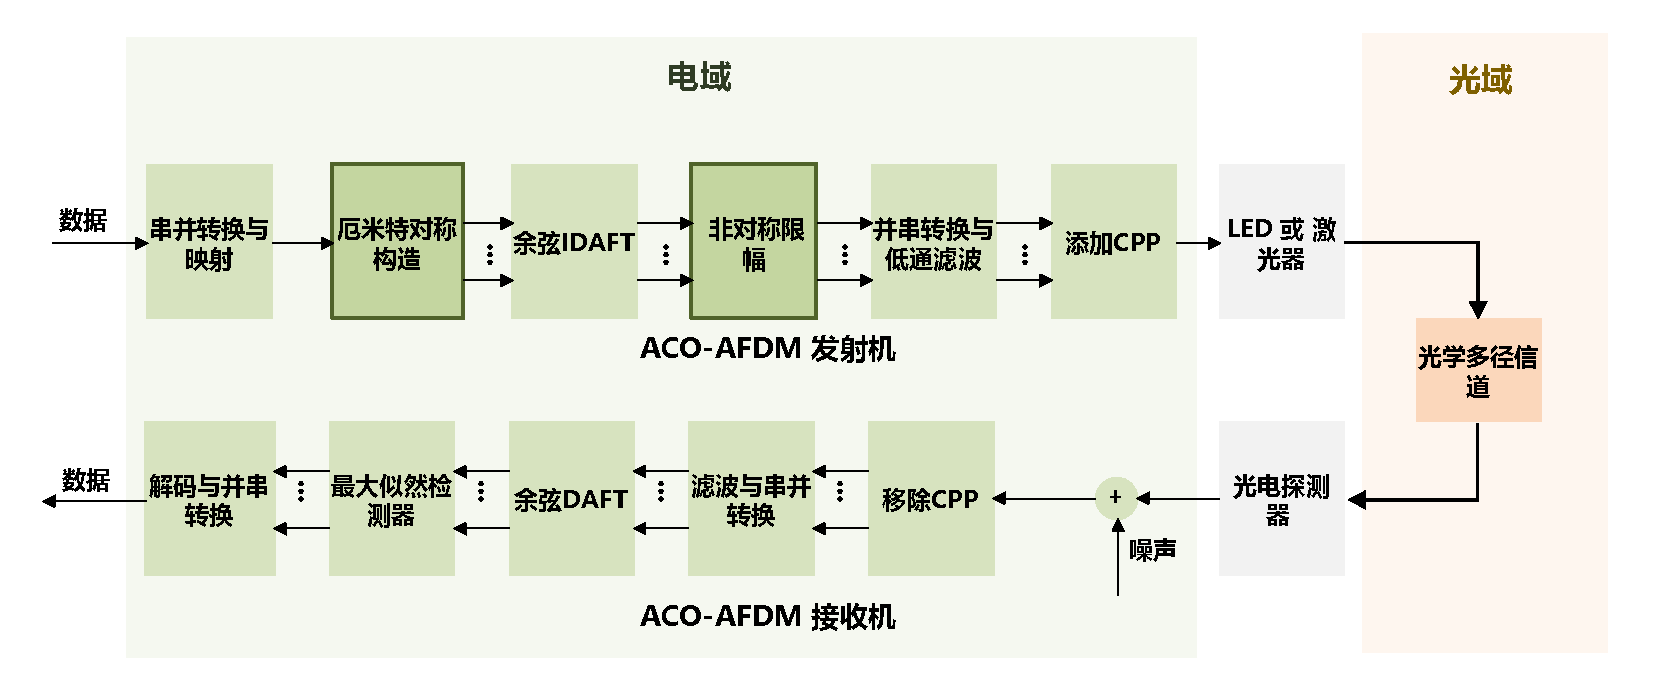
\includegraphics[width=1.0\linewidth]{figures/fig1_aco_afdm_system.pdf}
    \caption{ACO-AFDM 系统完整框图}
    \label{fig:aco_afdm_flow}
\end{figure}

从系统功能划分看，发射端主要完成比特映射、奇数位置加载、厄米特对称构造、AFDM 调制与非对称限幅；信道部分刻画低动态水下环境中的多径传播效应；接收端则完成前缀去除、变换域恢复、等效信道补偿与数据检测。通过这种设计，系统在满足光学发射物理约束的同时，可利用 AFDM 的结构优势增强对散射主导多径失真的适应能力。

\subsection{发射端信号生成与调制}
\label{subsec:aco_afdm_tx}

在发射端，输入比特首先映射为复数星座符号。为保证时域信号为实数，频域符号序列需满足厄米特对称条件。为避免限幅噪声落入承载数据信息的位置，ACO-AFDM 采用奇数子载波映射方式，即仅在奇数位置加载数据符号，偶数位置置零\cite{armstrongOFDMOpticalCommunications2009}。映射后的符号向量 $\mathbf{X}$ 表示为
\begin{equation}
    \mathbf{X} = [0, X_1, 0, X_3, \dots, X_{N/2-1}, 0, X_{N/2-1}^*, \dots, 0, X_3^*, 0, X_1^*]^T
\end{equation}

上述构造具有两个层面的作用。首先，厄米特对称保证经逆变换后得到的离散时域信号为实值，这是 IM/DD 系统可直接驱动光源的前提之一。其次，仅在奇数位置加载有效数据有助于在后续非对称限幅后将限幅噪声限制在偶数位置，从而避免其直接污染承载有效信息的变换域资源。因此，奇数子载波映射不仅是满足非负约束的技巧，也是一种围绕接收端可恢复性进行的结构化设计。

为将其映射到时域并保持实值特性，本文采用改进的余弦逆离散仿射傅里叶变换，其离散时域信号可表示为
\begin{equation}
    s[n] = \frac{1}{\sqrt{N}} \sum_{k=0}^{N-1} X[k] e^{j \frac{2\pi nk}{N}} \cos(2\pi c_1 n^2), \quad n=0,\dots,N-1
\end{equation}
其中，$c_1$ 为 DAFT 参数。本文令传统 AFDM 的第二参数 $c_2=0$，以保持半波反对称结构，即 $s[n] = -s[n+N/2]$。其矩阵形式可写为
\begin{equation}
    \mathbf{s} = \mathbf{C}\mathbf{F}^H \mathbf{X}
\end{equation}
其中，$\mathbf{C}$ 为由 $\cos(2\pi c_1 n^2)$ 构成的对角矩阵。

采用余弦型 DAFT 核的主要考虑在于，它能够在引入 AFDM 啁啾结构的同时保持时域实值信号特征，并与 ACO 机制所要求的半波反对称性质兼容。换言之，本文并不是简单将传统 AFDM 生硬套用于光学发射链路，而是围绕 IM/DD 约束对其变换核形式进行了有针对性的适配。参数 $c_1$ 的引入使信号在变换域中具备更适合多径分离的结构，而 $c_2=0$ 的设定则有助于维持 ACO 结构的可实现性和稳定性。

随后，对双极性时域信号进行非对称限幅，得到满足非负约束的发射信号
\begin{equation}
    s_{\mathrm{tx}}[n] = \max\{s[n], 0\}
\end{equation}
由于信号满足半波反对称性，限幅噪声仅分布于偶数子载波，不影响奇数子载波上的有效数据。最后，在每个信号块前添加长度为 $L_{\mathrm{cpp}}$ 的啁啾周期前缀，形成最终发射信号。

引入啁啾周期前缀的目的与传统循环前缀类似，都是为了抑制有限多径扩展导致的块间干扰，并为接收端的块处理恢复提供结构保证。不同之处在于，AFDM 调制后的信号具有啁啾相位特征，因此前缀设计需要与该结构保持一致。通过在块前添加适当长度的啁啾周期前缀，系统可在低动态多径条件下保持较稳定的块处理框架，从而为后续 DAFT 域恢复和信道均衡奠定基础。

\subsection{多径信道传播与接收端处理}
\label{subsec:aco_afdm_rx}

本文将低动态水下传播环境建模为具有 $P$ 条离散路径的时延抽头信道\cite{kaushalUnderwaterOpticalWireless2016a}。离散时间冲激响应可表示为
\begin{equation}
    h[n] = \sum_{i=1}^{P} h_i \delta[n-l_i]
\end{equation}
其中，$h_i$ 与 $l_i$ 分别表示第 $i$ 条路径的复增益和离散时延。接收端去除啁啾周期前缀后，接收信号向量为
\begin{equation}
    \mathbf{r} = \sum_{i=1}^{P} h_i \boldsymbol{\Pi}^{l_i}\mathbf{s}_{\mathrm{tx}} + \mathbf{w}
\end{equation}
其中，$\boldsymbol{\Pi}^{l_i}$ 为 $l_i$ 阶循环移位矩阵，$\mathbf{w}$ 为加性高斯白噪声。

上述模型反映了本文所关注的低动态场景的主要物理特征：路径之间的差异主要体现为传播时延和幅相响应差异，而由相对运动导致的时间快速变化可以近似忽略。因此，该信道更接近“准静态多径”而非“强时变双选择性”结构。尽管如此，当路径时延跨越多个采样间隔、且不同路径功率分布不均匀时，接收端仍会观察到显著的频率选择性衰落。这也是本章重点关注多径适应能力而非多普勒鲁棒性的原因。

接收端随后采用对应的余弦 DAFT 变换将信号恢复至仿射频域：
\begin{equation}
    Y[k] = \frac{1}{\sqrt{N}} \sum_{n=0}^{N-1} r[n] e^{-j \frac{2\pi nk}{N}} \cdot \frac{1}{\cos(2\pi c_1 n^2)}
\end{equation}
其矩阵形式为
\begin{equation}
    \mathbf{Y} = \mathbf{F}\mathbf{C}^{-1}\mathbf{r}
\end{equation}
由上述接收模型可知，系统在仿射频域中的恢复结果同时受多径卷积与限幅结构影响。在获得等效信道矩阵估计值 $\hat{\mathbf{H}}$ 后，可采用最大似然检测恢复原始数据符号。

从检测角度看，所提方案与传统 ACO-OFDM 的区别不仅体现在变换核不同，还体现在等效信道表示的结构差异。由于 AFDM 啁啾映射改变了路径时延在变换域中的投影形式，接收信号中的多径耦合不再表现为简单的傅里叶域子载波响应变化，而是体现为更具结构性的等效分布。这种结构差异为接收端进行更有针对性的均衡与检测提供了可能，也正是 ACO-AFDM 获得多径性能增益的关键所在。

\subsection{系统模型特点分析}
\label{subsec:aco_afdm_features}

综合发射端、信道与接收端结构，可以看出所提 ACO-AFDM 系统具有以下几个特点。

其一，系统在 IM/DD 架构下保持了实值非负发射的可实现性。通过厄米特对称、奇数位置加载和非对称限幅，发射端能够在不引入直流偏置的情况下满足光源驱动要求，并避免有效数据直接落入限幅噪声主分量所在位置。

其二，系统在保持 ACO 结构优势的同时，引入了 AFDM 的啁啾调制特性，使信号在面对低动态多径信道时能够在变换域中获得更适合描述路径结构的表示形式。相比传统 ACO-OFDM，这种结构更有利于减轻频率选择性衰落对局部资源位置的集中影响。

其三，系统的参数设计与接收端恢复过程存在显式耦合关系。特别是啁啾参数 $c_1$ 的选择不仅影响发射端变换实现，还直接决定接收端反变换的稳定性以及多径分量在 DAFT 域中的分布状态。因此，后续参数设计不能仅从数学可逆性出发，还需要同时考虑多径分离与实际检测性能。

基于上述特点，ACO-AFDM 并非简单地将 ACO 与 AFDM 两种机制进行形式叠加，而是在低动态多径 UWOC 场景下，围绕 IM/DD 发射约束、多径传播特性与接收恢复需求所形成的一种联合设计方案。

\section{ACO-AFDM 啁啾参数设计与全分集增益}
\label{sec:aco_afdm_params}

AFDM 的性能在较大程度上取决于啁啾参数设计。对于本文所提 ACO-AFDM 系统，参数 $c_1$ 的选择需同时满足逆变换稳定性与多径分离能力要求。由于本文采用余弦型 DAFT 核，参数设计不仅关系到信号在变换域中的分布形态，还直接影响接收端恢复过程中是否会出现数值不稳定或噪声增强现象。因此，有必要从奇异点规避与多径分离两个方面对其进行分析。

\subsection{奇异点规避准则}
\label{subsec:singularity_avoidance}

由接收端恢复公式可知，分母项中包含 $\cos(2\pi c_1 n^2)$。为避免逆变换过程中出现零点或过小值导致的噪声放大，需要满足
\begin{equation}
    2\pi c_1 n^2 \neq \frac{\pi}{2} + m\pi, \quad m \in \mathbb{Z}
\end{equation}
等价地，有
\begin{equation}
    c_1 \neq \frac{1/4 + m/2}{n^2}, \quad m \in \mathbb{Z}
    \label{eq:singularity_condition}
\end{equation}
因此，在参数选择时应剔除上述无效取值点。

这一约束的物理意义在于，余弦型 DAFT 核中包含的幅度调制项若在某些离散采样点附近接近零值，将使接收端在执行逆变换时对应位置的噪声被显著放大，进而导致整体检测性能恶化。换言之，即使某些参数在理论上并不破坏映射关系，只要其使 $\cos(2\pi c_1 n^2)$ 过小，也会降低系统实现稳定性。因此，奇异点规避不仅是数学层面的可逆性要求，也是工程实现中的数值稳健性要求。

在实际设计中，还应注意“避开严格零点”与“避开过小值区域”之间存在差异。前者保证逆变换在理论上可定义，后者则更贴近有限精度运算和实际噪声环境下的性能需求。因而，在候选参数搜索时，通常需要为 $\cos(2\pi c_1 n^2)$ 设定适当的安全裕量，而不是仅仅排除解析意义下的奇异取值点。

\subsection{多径分离与分集准则}
\label{subsec:multipath_separation}

为实现多径分量在 DAFT 域中的有效分离，需要考察路径时延引起的位置偏移。对于第 $i$ 条路径，其在 DAFT 域中的对称偏移位置可表示为
\begin{equation}
    \mathrm{loc}_i = (2N c_1 l_i)_N, \quad \mathrm{loc}_i^{\prime} = (-2N c_1 l_i)_N
\end{equation}
其中，$(\cdot)_N$ 表示模 $N$ 运算。

为避免不同路径在 DAFT 域中发生位置重叠，对于任意 $i \neq j$，需满足
\begin{equation}
    \{ \mathrm{loc}_i, \mathrm{loc}_i^{\prime} \} \cap \{ \mathrm{loc}_j, \mathrm{loc}_j^{\prime} \} = \emptyset
\end{equation}
若最大时延扩展为 $l_{\max}$，则为保证全部偏移范围不超过 DAFT 域长度 $N$，应满足
\begin{equation}
    4N c_1 l_{\max} \leq N
\end{equation}
由此得到参数边界
\begin{equation}
    0 < c_1 \leq \frac{1}{4 l_{\max}}
    \label{eq:c1_boundary}
\end{equation}
当 $c_1$ 同时满足式(\ref{eq:singularity_condition}) 与式(\ref{eq:c1_boundary}) 时，系统可在保证逆变换稳定性的同时提高对多径分量的分离能力。

上述准则说明，啁啾参数并不是越大越好或越小越好，而是需要在“增强路径可分辨性”和“控制变换域重叠风险”之间取得平衡。当 $c_1$ 过小时，不同路径在 DAFT 域中的偏移量较小，可能不足以体现 AFDM 对多径结构的区分优势；当 $c_1$ 过大时，路径对应响应又可能由于周期性折返而发生重叠，从而削弱系统的结构化表示能力。因此，合理参数区间本质上来自多径分离需求与有限离散维度约束的共同作用。

从分集利用角度看，若不同路径在 DAFT 域中能够保持较好的可区分性，则接收端在检测时更容易利用多径传播所提供的结构差异，而不是将其完全视作干扰源。这意味着，多径分量不再只是造成性能下降的失真项，也可能在合理波形设计下转化为可被利用的分集资源。本文所讨论的参数设计准则，正是为了使 ACO-AFDM 在低动态多径场景中尽可能保留这种结构性收益。

\subsection{参数设计的工程含义与取值权衡}
\label{subsec:param_tradeoff}

除上述理论约束外，参数 $c_1$ 的实际选取还应结合系统维度、最大时延扩展估计精度以及接收端复杂度进行综合考虑。对于较小的系统维度 $N$，可供选择的离散参数空间相对有限，若同时要求严格规避奇异点和路径重叠，则可行参数集合可能明显收缩；而当 $N$ 较大时，系统具有更细粒度的参数调节空间，但实现复杂度和前缀开销也可能随之上升。

此外，参数设计通常依赖对最大时延扩展 $l_{\max}$ 的先验估计。若该估计偏小，则依据式(\ref{eq:c1_boundary}) 选择的参数可能在真实信道下导致路径响应重叠；若估计偏大，则参数设置又可能过于保守，使 AFDM 的结构优势不能充分发挥。因此，在实际系统中，参数设计往往需要在鲁棒性与性能增益之间留出一定裕量。

从实现角度看，本文采用的参数设计并不追求全局最优，而是强调“可实现、可解释、与场景相适配”的选择原则。对于硕士论文层面的系统设计而言，这种基于物理约束和结构分析得到的参数准则具有较好的理论完整性与工程合理性，也为后续仿真设置提供了依据。

\section{仿真结果与分析}
\label{sec:aco_afdm_sim}

为验证所提 ACO-AFDM 方案在低动态多径水下场景中的性能，本节采用蒙特卡罗方法开展仿真，并与 ACO-OFDM、U-OFDM 以及 DCO-OFDM 进行对比\cite{dissanayakeComparisonACOOFDMDCOOFDM2013, fernandoFlipOFDMUnipolarCommunication2011}。

在仿真设置中，各方案均采用 $N=256$ 的子载波配置与 16-QAM 调制方式，并在接收端采用最大似然检测。针对所提 ACO-AFDM 方案，依据参数设计准则取 $c_1 = 1/(8l_{\max})$。水下多径信道建模为具有指数衰减功率延迟分布的离散瑞利信道。

上述设置旨在保证不同方案之间的可比性。统一的调制阶数和资源维度使性能差异主要来源于波形结构及其对多径传播的适应能力，而不是由参数不一致带来的额外偏差。同时，采用指数衰减型功率延迟分布能够较好反映低动态散射环境中“主路径较强、延迟路径逐步衰减”的典型传播特征，从而使仿真结论更贴近本文讨论的代表性应用条件。

\begin{figure}[htbp]
    \centering
    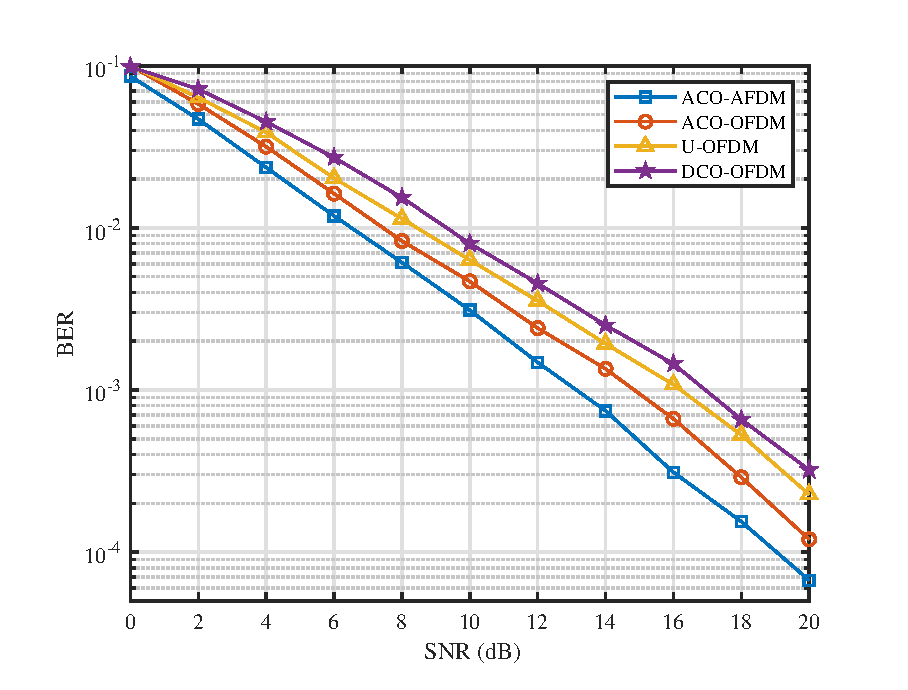
\includegraphics[width=0.85\linewidth]{figures/fig2_aco_afdm_ber_2path.eps}
    \caption{不同多载波方案在两径信道下的误码率性能对比}
    \label{fig:ber_comparison_2path}
\end{figure}

图~\ref{fig:ber_comparison_2path} 给出了最大时延扩展 $l_{\max}=10$ 采样周期时，各方案的 BER 与 SNR 关系曲线。由图可见，所提 ACO-AFDM 方案在整个观测 SNR 区间内均优于对比方案。在 $\mathrm{BER}=10^{-3}$ 附近，相较于 ACO-OFDM 可获得约 2 dB 的性能增益，说明所提方案在低动态多径条件下具有较好的误码率性能。

这一结果表明，在低动态 UWOC 中，系统性能的关键不完全取决于发射信号是否满足非负约束，还与波形对多径传播的适应能力密切相关。ACO-OFDM、U-OFDM 与 DCO-OFDM 虽然都能够实现单极性光信号传输，但它们在本质上仍主要依赖傅里叶域正交结构，因此当时延扩展引起明显频率选择性衰落时，部分资源位置会更易遭受性能退化。相比之下，ACO-AFDM 通过 DAFT 域中的结构化表示，使接收端能够更有效地应对多径导致的能量分散与局部深衰落问题，因此在相同信噪比条件下表现出更低的误码率。

需要注意的是，在较低 SNR 区间内，各方案之间的差距相对有限。这是因为噪声在此时仍是影响误码性能的主要因素，波形结构优势尚未充分显现；随着 SNR 提高，噪声影响逐渐减弱，信道结构与波形匹配关系开始主导系统性能，此时 ACO-AFDM 相对于传统光 OFDM 体制的优势更加明显。这一趋势与本文前述理论分析相一致。

\begin{figure}[htbp]
    \centering
    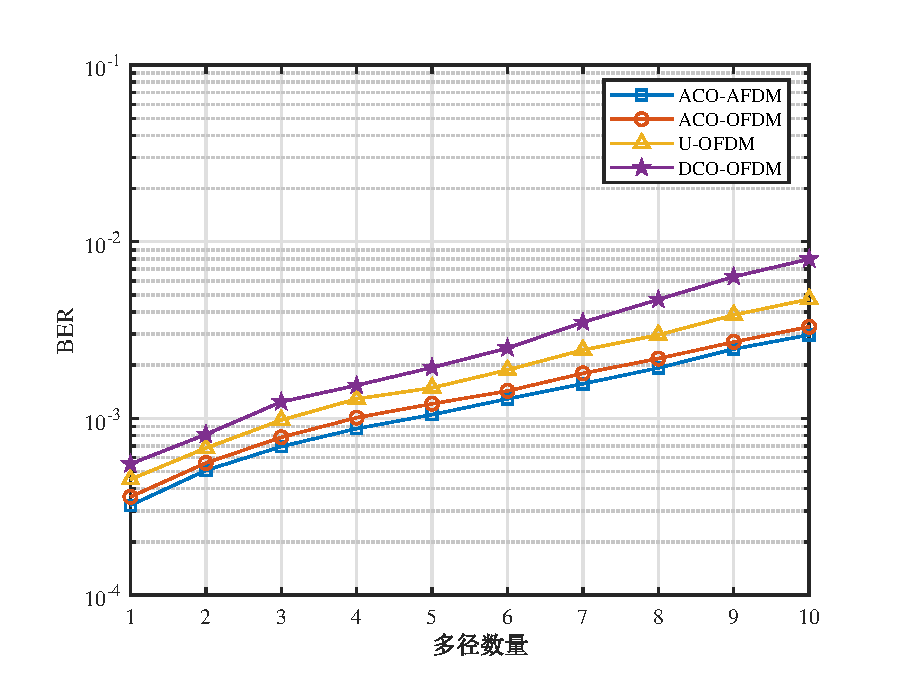
\includegraphics[width=0.85\linewidth]{figures/fig3_aco_afdm_ber_multipath.eps}
    \caption{多径路径数量对系统误码率性能的影响}
    \label{fig:multipath_robustness}
\end{figure}

图~\ref{fig:multipath_robustness} 给出了固定 $\mathrm{SNR}=16\,\mathrm{dB}$ 条件下，系统误码率随多径路径数变化的结果。由图可见，随着路径数量增加，传统 ACO-OFDM 与 U-OFDM 方案的误码率明显恶化，而 ACO-AFDM 的性能退化相对较缓。这表明所提方案对低动态水下多径传播具有更好的适应能力。

从机理上看，路径数增加意味着系统接收到更多延迟分量，频率选择性衰落程度加深，且不同路径之间的叠加关系更加复杂。对于传统光 OFDM 方案而言，这通常意味着子载波间信道增益差异增大、部分频率位置出现更严重的深衰落，从而使整体检测性能明显下降。而对于 ACO-AFDM，由于啁啾参数设计使多径响应在 DAFT 域中更具结构性，新增路径带来的影响并不完全等价于“更多随机干扰”，而是在一定程度上仍可通过结构化表示进行处理，因此其误码率退化速度较慢。

上述结果还说明，所提方案的性能优势并非仅体现在单一固定信道条件下，而是在多径复杂度变化时仍具有一定稳健性。这一点对于实际 UWOC 系统尤为重要，因为不同海域环境、不同水体浑浊程度以及不同收发几何条件下的路径数量和功率分布往往并不稳定。若一种传输方案仅在理想双径条件下有效，其工程适用性将受到明显限制；而 ACO-AFDM 在多路径数变化下仍保持相对稳定的性能表现，说明其更适合作为低动态多径场景下的候选物理层方案。

\subsection{结果讨论}
\label{subsec:aco_afdm_discussion}

综合上述仿真结果可以看出，所提 ACO-AFDM 方案在低动态多径 UWOC 场景下相较传统光 OFDM 方案具有更好的 BER 性能和多径鲁棒性。其优势主要来自以下几个方面：首先，ACO 结构保证了发射信号能够满足 IM/DD 架构的非负实值约束，并维持较好的光功率利用效率；其次，AFDM 啁啾映射增强了系统对多径传播结构的适应能力，使信号在变换域中的表示更有利于路径分离与检测；再次，合理的啁啾参数设计使系统在逆变换稳定性与多径分离能力之间取得了较好平衡。

进一步来看，所提方案的价值并不仅在于相较 ACO-OFDM 获得若干分贝的性能增益，更在于其揭示了一条适用于低动态 UWOC 的设计思路：即在 IM/DD 非负约束不可回避的前提下，可以通过对波形结构进行重新设计，而不是仅依赖传统 OFDM 框架下的局部修正，来提升系统对散射主导多径环境的适应能力。这种思路与本文全文所强调的“围绕场景特征对 AFDM 进行适配”的主线保持一致。

从本章研究过程可以进一步归纳出，所提方案在系统层面完成了三个相互关联的工作：一是在模型构建上，将奇数子载波映射、厄米特对称、余弦型 AFDM 调制与非对称限幅机制统一到 IM/DD 发射框架中，建立了适用于低动态多径水下光链路的收发模型；二是在参数设计上，围绕余弦型 DAFT 核分析了奇异点规避与多径分离条件，明确了啁啾参数的选取依据；三是在性能层面，通过 BER 与多径鲁棒性仿真验证了该方案在满足非负实信号约束的同时，能够较好提升系统对低动态多径传播的适应能力。由此可见，ACO-AFDM 并非对既有光 OFDM 结构的简单替换，而是面向低动态 UWOC 场景所形成的一种具有明确物理约束、参数依据与性能支撑的联合设计方案。

当然，所提方案也存在一定局限性。首先，本文仿真主要基于离散多径模型与理想同步假设展开，尚未进一步考虑更复杂的发射器非线性、接收器响应带宽限制及更强随机湍流扰动等因素；其次，参数设计在一定程度上依赖对最大时延扩展的先验估计，当信道统计特性明显偏离设计条件时，系统性能可能受到影响；再次，本文重点讨论误码率性能，对硬件实现复杂度、前缀开销和峰均功率比等工程指标尚未展开更深入分析。这些问题都可作为后续研究的拓展方向。
